\documentclass{article}
\usepackage{graphicx}
\usepackage[margin=1.5cm]{geometry}
\usepackage{amsmath}

\begin{document}

\title{Tuesday Reading Assessment: Unit 1, Ohm's Law and Batteries, DC Circuits and Power}
\author{Prof. Jordan C. Hanson}

\maketitle

\section{Memory Bank}

\begin{itemize}
\item $V = IR$ ... Ohm's Law
\item $P = IV$ ... Relationship between power, voltage, and current
\item $V_{\rm terminal} = \epsilon - Ir$ ... For a battery, the terminal voltage is the emf or ideal voltage, minus the current times the internal resistance.
\end{itemize}

\section{Batteries and Power}

\begin{enumerate}
\item (a) What is the power consumption of a 24 V system that draws 0.5 A of current? (b) If a different system operates at 12 V, and has a total resistance of 50$\Omega$, what is the power consumption? \\ \vspace{1cm}
\item Suppose a a battery is connceted in series with a resistor (Fig. \ref{fig:dura}).  The $\epsilon$, or emf of the battery is 1.5 V.  The resistor $R$ is 50$\Omega$.  The current measured to be 0.0285 A.  (b) What is $r$, the internal resistance? (c) If another 50$\Omega$ resistor was added \textit{in parallel}, what would be the new current?
\begin{figure}[ht]
\centering
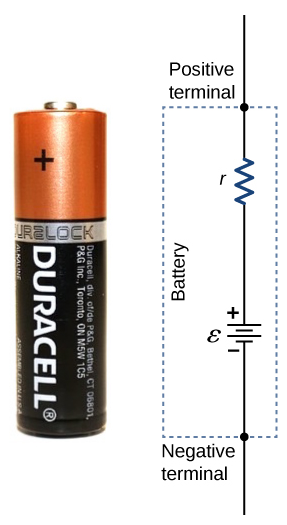
\includegraphics[width=0.15\textwidth]{duracell.png}
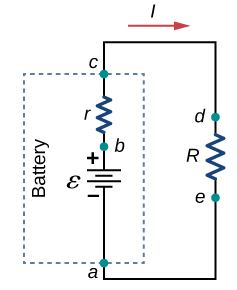
\includegraphics[width=0.15\textwidth]{duracell2.png}
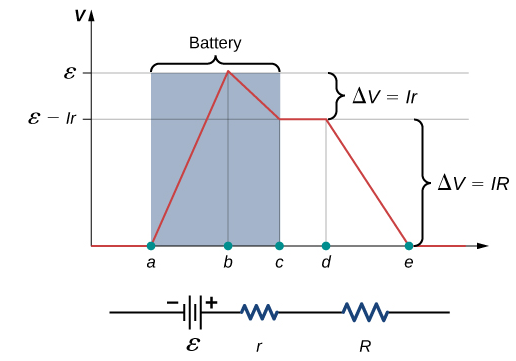
\includegraphics[width=0.3\textwidth]{duracell3.png}
\caption{\label{fig:dura} (Left) A battery is similar to a chemical capacitor, but keeps constant a constant voltage $\epsilon$ called the emf. (Middle) However, a more accurate model is that the battery has some intrinsic or internal resistance $r$.  (Right) Thus, the measured voltage $V_{\rm terminal}$ does not reach the idea emf for a given current $I$.}
\end{figure}
\end{enumerate}

\end{document}
